\subsection{Понятие функции многих переменных} \label{sec:1.2}

Начнем с определения функции одной переменной.

Если каждому числу $x$ из множества $\mathbb{E}$, которое является подмножеством действительных чисел $\mathbb{R}$, соответствует число $y$ из множества $Y$, также являющегося подмножеством $\mathbb{R}$ в соответствии с правилом $f$, то говорят, что на множестве $\mathbb{E}$ задана функция $y = f(x)$. Множество $\mathbb{E}$ называют областью определения функции, а $Y$ — множеством её значений.\\

Функция нескольких переменных определяется аналогично, только вместо одного числа используются несколько независимых переменных.

\begin{tbox*}{Определение функции k независимых переменных}
	Если каждому вектору $\vec{x} = (x_1, x_2, ..., x_k)$ из множества $\mathbb{E} \subset \mathbb{R}^k$ соответствует число $y$ из множества $Y \subset \mathbb{R}$ по правилу $f$, то на множестве $\mathbb{E}$ задана функция нескольких переменных, которую обозначают как $y = f(\vec{x})$ или $y = f(x_1, x_2, ..., x_k)$.

	Здесь $x_1, x_2, ..., x_k$ — независимые переменные (аргументы функции), а $y$ — зависимая переменная.

	Множество $\mathbb{E} \subset \mathbb{R}^k$ называют областью определения функции, а множество $Y \subset \mathbb{R}$ — её множеством значений.
\end{tbox*}

\subsubsection{Частные случаи функций многих переменных}
Рассмотрим функции двух и трех переменных. Для функции двух переменных:

\begin{itemize}
	\item Если $k=2$, то $y = f(x_1, x_2)$, что записывается как $z = f(x, y)$;
	\item Если $k=3$, то $y = f(x_1, x_2, x_3)$, что записывается как $w = f(x, y, z)$.
\end{itemize}

Особенно важна функция двух переменных $z = f(x, y)$, где $x$ и $y$ — независимые переменные. Область определения этой функции — множество точек $(x, y)$, принадлежащих некоторому подмножеству $\mathbb{E} \subset \mathbb{R}^2$. Зависимая переменная $z$ принимает значения из множества $Z \subset \mathbb{R}$, которое откладывается по вертикальной оси в пространстве XYZ.

По определению функции, каждой паре $(x, y) \in \mathbb{E}$ ставится в соответствие единственное значение $z$ по закону $f$. Это означает, что функция двух переменных имеет графическое представление в виде поверхности в пространстве. Эта поверхность состоит из всех значений функции во всех точках области определения $\mathbb{E}$.

\noindent
\begin{minipage}{\linewidth}
	\begin{minipage}{0.6\linewidth}
		\begin{tbox*}{Параболоид вращения (\Cref{fig:1.2.1.1})}
			\[\boxed{z = x^2 + y^2}\]
			О.О. $(x, y) \in \mathbb{R}$, $z \geqslant 0$ - множество значений
		\end{tbox*}
	\end{minipage}
	\begin{minipage}{0.35\linewidth}
		\begin{figure}[H]
			\centering
			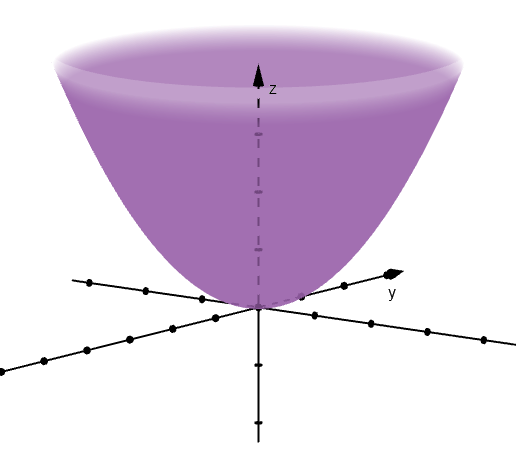
\includegraphics[width=0.9\linewidth]{image/screenshot004.png}
			\caption{Параболоид}
			\label{fig:1.2.1.1}
		\end{figure}
	\end{minipage}
\end{minipage}
\begin{minipage}{\linewidth}
	\begin{minipage}{0.6\linewidth}
		\begin{tbox*}{Коническая поверхность (\Cref{fig:1.2.1.2})}
			\[\boxed{z^2 = x^2 + y^2}\]

			-- это неявно заданная функция. Выразим из уравнения $z$, $z = \pm \sqrt{x^2 + y^2}$ - получаем две явно заданные функции:
			\begin{enumerate}
				\item $\boxed{z = \sqrt{x^2 + y^2}}$, $(x, y) \in \mathbb{R}^2$, $z \geqslant 0$
				\item $\boxed{z = -\sqrt{x^2 + y^2}}$, $(x, y) \in \mathbb{R}^2$, $z \leqslant 0$
			\end{enumerate}
		\end{tbox*}
	\end{minipage}
	\begin{minipage}{0.35\linewidth}
		\begin{figure}[H]
			\centering
			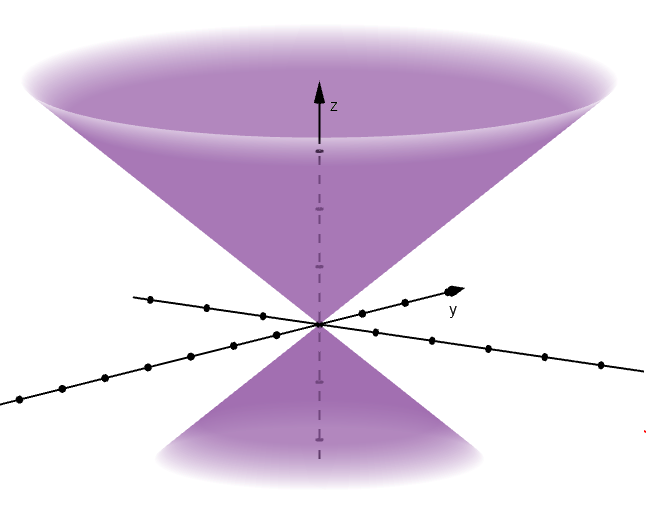
\includegraphics[width=0.9\linewidth]{image/screenshot005.png}
			\caption{Коническая поверхность}
			\label{fig:1.2.1.2}
		\end{figure}
	\end{minipage}
\end{minipage}
\begin{minipage}{\linewidth}
	\begin{minipage}{0.6\linewidth}
		\begin{tbox*}{Сфера с цетром в начале (\Cref{fig:1.2.1.3})}
			\[\boxed{x^2 + y^2 + z^2 = R^2}\]

			Функция $z = \sqrt{R^2 - x^2 - y^2}$ задает верхнюю половину сферы. Здесь область определения $R^2 -x^2 - y^2 \geqslant 0 \Rightarrow x^2 + y^2 \leqslant R^2$ - круг радиуса $R$, а множество значений $0 \leqslant z \leqslant R$.\\

			Функция $z = -\sqrt{R^2 - x^2 - y^2}$ задает нижнюю половину сферы, область определения $x^2 + y^2 \leqslant R^2$, а множество значений $-R \leqslant z \leqslant 0$.\\

			\textbf{Замечание: } Функции, большего числа переменных, не имеют геометрического изображения.
		\end{tbox*}
	\end{minipage}
	\begin{minipage}{0.35\linewidth}
		\begin{figure}[H]
			\centering
			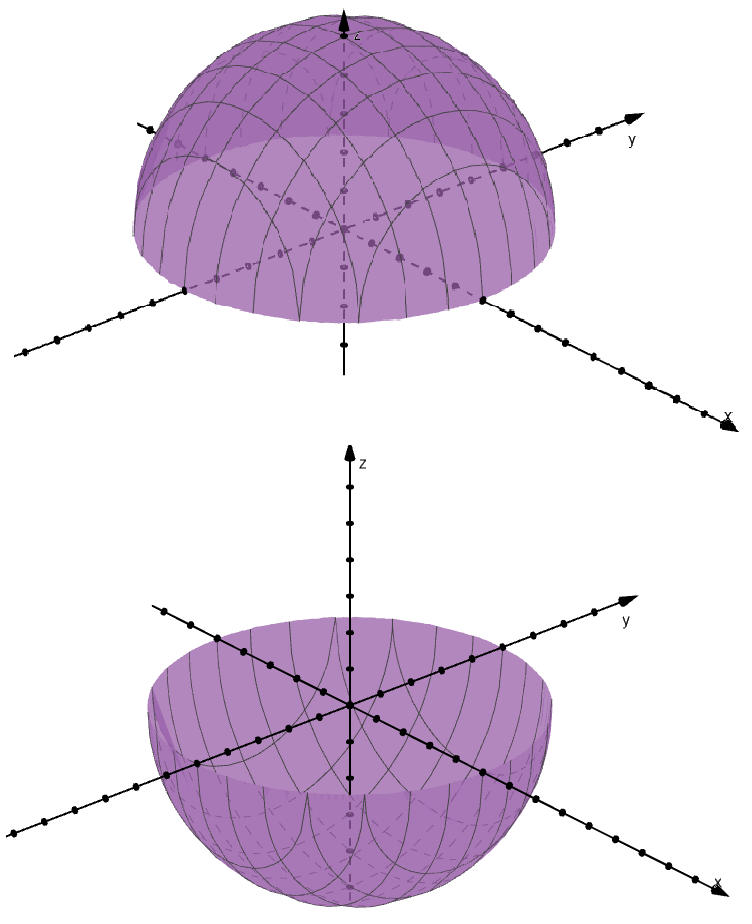
\includegraphics[width=0.9\linewidth]{image/screenshot007.png}
			\caption{Сфера с цетром в начале}
			\label{fig:1.2.1.3}
		\end{figure}
	\end{minipage}
\end{minipage}
